%%
%% AAAI-27 Artificial Intelligence for Social Impact (AISI) Special Track
%% Anonymous submission. MERGED DRAFT: AIware 2026 (rejected) kept complete
%% and unmodified as the base system paper; the AISI evaluation work is
%% added as new sections (Measuring the Data Gap, Human Annotation and
%% Agreement, Tagging Methods, Evaluation) and appended to Limitations.
%% Built against the official AAAI-27 Author Kit (aaai2027.sty /
%% aaai2027.bst), copied alongside this file.
%%
\documentclass[letterpaper]{article}
\usepackage[submission]{aaai2027}
\usepackage[hyphens]{url}
\usepackage{graphicx}
\urlstyle{rm}
\def\UrlFont{\rm}
\usepackage{natbib}
\usepackage{caption}
\frenchspacing
\usepackage{booktabs}
\pdfinfo{
/TemplateVersion (2027.1)
}

\setcounter{secnumdepth}{1}

\title{Bridging the Data Gap: A Human-Validated Pipeline for\\
Culturally Aligned Topic Detection in Black Media}

\author{
    Anonymous Submission
}
\affiliations{
}

\begin{document}

\maketitle

\begin{abstract}
In the age of generative artificial intelligence, equitable AI development
requires training data that reflects the full breadth of human experience,
yet Black media publications remain systematically absent from major news
corpora such as C4 and Common Crawl. This absence embeds structural blind
spots into language models and limits their cultural alignment for Black
communities. We present a modular, open-source pipeline that continuously
scrapes, normalizes, and thematically annotates articles from ten prominent
Black media publications on a rolling monthly horizon, delivering
approximately 1,200 articles per cycle tagged against a curated taxonomy of
twelve social-conflict topics. To move beyond pipeline description, we
construct a 400-article human-annotated benchmark across two independent
annotators and conduct a rigorous comparative evaluation of six tagging
approaches: keyword matching, semantic similarity, three hybrid variants,
and a supervised classifier trained on sentence embeddings. We establish a
human agreement baseline through expert re-labeling and inter-annotator
agreement analysis, finding macro Cohen's kappa of 0.33 to 0.38, then show
that our best method, a per-topic logistic regression combining embeddings
with keyword and semantic signals, reaches 77 to 91 percent of that
baseline with a macro F1 of 0.322 and kappa of 0.297 under a leak-free
cross-annotator validation protocol, a gap over the best honest baseline
that survives a paired bootstrap significance test. We release the
pipeline code, taxonomy, and annotation metadata to support replication
and extension to other under-represented media ecosystems.
\end{abstract}

\section{Introduction}

Large language models are heavily shaped by their training data, and
Black media corpora are significantly absent from mainstream AI training
datasets, reflecting broader patterns of exclusion and misrepresentation
in AI data collection and model development \citep{bender2021}. Even
with nonprofit web archives such as Common Crawl \citep{baack2024}
providing the raw material for datasets like C4, the Colossal Clean
Crawled Corpus, a filtered, cleaned web-text corpus used to pretrain the
widely used T5 family of language models \citep{raffel2020}, there is
currently no widely recognized corpus explicitly curated as a Black
media corpus; instead, existing critiques indicate that downstream
filtering can exclude content associated with Black authors and other
marginalized groups \citep{baack2024}. This persistent
underrepresentation of Black media in foundational training corpora
contributes to the cultural misalignment increasingly observed in AI
systems, particularly in how these systems handle socially sensitive
issues affecting Black communities, where gaps in representation can
produce distorted, incomplete, or culturally insensitive responses
\citep{tao2024}.

The corpus-level absence described above is not only asserted in the
literature; we measure it directly. Auditing the Common Crawl snapshot
underlying C4, we find that nine of the ten Black media publications
monitored in this work have a combined footprint of fewer than 8,000 raw
captures, several orders of magnitude below single mainstream outlets
such as nytimes.com \citep{dodge2021}; the tenth, Capital B News,
founded in 2022, cannot appear in the snapshot at all
(Section~\ref{sec:gap}). We monitor these ten publications through a
continuously running collection pipeline, an earlier version of which
responded to this same absence by building collection infrastructure
for community media. But collection alone leaves a critical question
unanswered, one that reviewers of such systems rightly press: are the
produced topic labels reliable enough for downstream research or
model-development use? A pipeline that tags articles with unvalidated
heuristics produces a dataset whose labels cannot be trusted, and an
untrustworthy dataset serves the community it documents poorly.

This paper answers that question for our pipeline, and in doing so
offers a template for answering it in other low-resource media
ecosystems. We make four contributions:

\begin{enumerate}
\item \textbf{An extended collection pipeline.} We expand coverage to
ten Black media publications, scraped on a rolling monthly horizon
($\sim$1{,}200 articles per cycle), tagged against a twelve-topic
social-conflict taxonomy, fully automated via CI/CD
(Section~\ref{sec:architecture}).
\item \textbf{A human-annotated benchmark with an agreement baseline.}
Two independent annotators labeled 200 articles each; expert re-labeling
of all 400 yields inter-annotator agreement of macro $\kappa =
0.33$--$0.38$, establishing the human baseline against which any
automated tagger must be read (Section~\ref{sec:annotation}).
\item \textbf{A leak-free comparative evaluation of six tagging
methods.} We compare keyword matching, semantic similarity, and hybrid
variants under cross-annotator validation, and document a
threshold-tuning leak whose correction reduces apparent performance by
0.07 macro F1 (Section~\ref{sec:eval}).
\item \textbf{A validated supervised classifier.} A per-topic logistic
regression over sentence embeddings, keyword, and semantic signals
reaches macro F1 0.322 and $\kappa$ 0.297, 77--91\% of the human
baseline, and is adopted as the pipeline's production tagger
(Sections~\ref{sec:methods}--\ref{sec:eval}).
\end{enumerate}

We frame this system as a foundational, incrementally validated pipeline
rather than a finished large-scale resource, and we prioritize
transparency about data sparsity and annotation difficulty over scale or
performance claims throughout (Section~\ref{sec:limitations}).

\section{Background and Motivation}
\label{sec:background}

The performance, safety, and fairness of generative AI systems are
fundamentally shaped by the composition of their training data.
\citet{bender2021} demonstrate that large language models trained
predominantly on internet text inherit the biases of dominant online
demographics, skewing toward English, toward Western cultural norms, and
toward the perspectives of groups that are over-represented in digital
publishing. \citet{blodgett2020} trace a direct line from corpus
composition choices to downstream disparities in NLP system performance
across demographic groups, arguing that these disparities are not
incidental engineering failures but consequences of how training data is
assembled. \citet{dodge2021} further document the extent to which
commonly used web crawls, including C4, the Colossal Clean Crawled
Corpus that underpins many modern LLMs, contain systematic demographic
biases introduced by domain-level filtering choices.

Cultural alignment, defined as the goal of building AI systems that
understand and respect the communicative norms, values, and lived
experiences of diverse communities, requires rethinking existing data
infrastructures, including what is collected, annotated, and
benchmarked \citep{hershcovich2022}. For communities whose media and
linguistic output is absent from standard corpora, improving cultural
alignment requires first building the data pipelines that make their
content accessible at scale.

\subsection{Limitations of ``Mainstream'' News Corpora}

Large open news corpora provide convenient baselines for NLP
benchmarking but exhibit well-documented source-diversity problems. The
GDELT project \citep{gdelt2026} indexes news from millions of articles
worldwide, but its reliance on widely accessible online sources means
that coverage is skewed toward major, often English-language outlets
rather than a balanced sample of all media ecosystems. All the News 2.0
\citep{thompson2020} and CC-News \citep{mackenzie2020} are similarly
constructed from web crawls that focus on large, high-visibility news
sites, offering limited coverage of smaller or lower-traffic domains,
and RealNews \citep{zellers2019} is drawn from a comparably narrow set
of mainstream sources, all exhibiting limited transparency and uneven
editorial diversity in source selection \citep{gruppi2020}. Specialized
datasets such as MedMCQA \citep{pal2022}, LegalBench \citep{guha2023},
and FinancialPhraseBank \citep{malo2014} address vertical domain gaps
but have no analogue for community or ethnic press coverage. The
consequence is that the corpora used to train and evaluate AI systems
for general-audience tasks systematically exclude the media output of
communities that are already under-served by those systems.

\subsection{Gap in Automated Monitoring Tools}

Along with limitations in existing corpora, there are also gaps in
automated tooling and support for niche dataset creation. Existing
media-monitoring services like Meltwater \citep{meltwater2026}, Cision
\citep{cision2024}, and the GDELT Analysis Service
\citep{gdeltanalysis2025} are proprietary, costly, and not designed to
export clean research datasets. Open alternatives such as NewsAPI
\citep{newsapi2026} or Media Cloud \citep{mediacloud2020} provide useful
APIs but do not index the Black press at sufficient depth or recency. No
open-source, self-hosted tool exists that (a) targets this specific
publication set, (b) applies a sociologically grounded topic taxonomy,
and (c) runs fully automated on free CI/CD infrastructure. The absence
of such tooling is itself a barrier to AI alignment research: without
accessible, regularly updated data, it is difficult to sustainably study
representation gaps, construct evaluation benchmarks, or gather
fine-tuning corpora at the pace that AI development demands.

\section{Measuring the Data Gap}
\label{sec:gap}

Earlier presentations of this pipeline asserted that its sources are
missing from mainstream corpora; here we measure it. C4
\citep{raffel2020} was filtered from the Common Crawl snapshot
CC-MAIN-2019-18. We queried the Common Crawl index for every capture of
each of our ten publication domains in that snapshot
(Table~\ref{tab:audit}). Because C4's filters (English-only,
deduplication, blocklists, length heuristics) only \emph{remove} pages,
these counts upper-bound each domain's possible C4 presence.

\begin{table}[t]
\centering
\small
\begin{tabular}{lr}
\toprule
Domain & Captures in CC-MAIN-2019-18 \\
\midrule
blavity.com        & 3{,}774 \\
theroot.com        & 1{,}291 \\
ebony.com          &   911 \\
thegrio.com        &   881 \\
essence.com        &   407 \\
newsone.com        &   203 \\
afrotech.com       &   186 \\
21ninety.com       &   113 \\
capitalbnews.org   &     0 \\
travelnoire.com    &   n/a\textsuperscript{*} \\
\midrule
Combined (measured) & 7{,}766 \\
\bottomrule
\end{tabular}
\caption{Presence of our ten publication domains in the Common Crawl
snapshot from which C4 was built. \textsuperscript{*}Index query
unresolved at submission time. For scale, \emph{nytimes.com} is among
the largest domains in all of C4 \citep{dodge2021}. \emph{Capital B News}
(founded 2022) post-dates the snapshot entirely.}
\label{tab:audit}
\end{table}

The combined measured footprint of nine of our ten domains, 7,766 raw
captures before C4's aggressive filtering, is several orders of
magnitude smaller than that of a single mainstream outlet. Any
publication founded after a corpus's snapshot date is structurally
invisible to models trained on it, and community media skews young.
Continuous collection, not one-time archival, is therefore the
appropriate remedy, which is what the pipeline provides.

\section{System Architecture and Approach}
\label{sec:architecture}

Building datasets for the cultural alignment of AI requires
infrastructure that is not only technically sound but also
reproducible, low-cost, and extensible to new data ecosystems without
prohibitive engineering overhead. The pipeline described here is
designed with these requirements in mind: its outputs can serve as
evaluation benchmarks for testing the cultural competence of generative
AI systems, as fine-tuning corpora for models intended for deployment in
Black communities, or as raw material for framing and coverage studies
that aim to characterize the data gap.

The pipeline (Figure~\ref{fig:pipeline}) consists of four decoupled
stages executed sequentially by a single orchestrator
(\texttt{run.py}): Scrape $\rightarrow$ Analyze $\rightarrow$ Report
$\rightarrow$ Deliver. Each stage reads from and writes to the
\texttt{outputs/} directory, enabling any stage to be re-run
independently.

\begin{figure}[t]
\centering
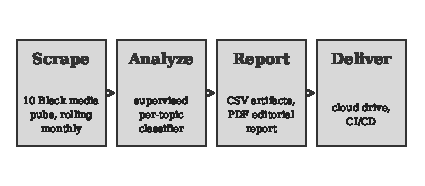
\includegraphics[width=0.9\columnwidth]{figures/fig_pipeline.pdf}
\caption{The four-stage pipeline. This paper's contribution is the
validation of the \emph{Analyze} stage: the supervised classifier
adopted there (Sections~\ref{sec:methods}--\ref{sec:eval}) is the best
of six methods evaluated against a 400-article human benchmark.}
\label{fig:pipeline}
\end{figure}

\subsection{Stage 1: Scraping}

Each of the media outlets requires a distinct scraping strategy due to
differences in their technology stack (Table~\ref{tab:sources}).

\begin{table}[t]
\centering
\small
\begin{tabular}{lll}
\toprule
Publication & Method & Fallback \\
\midrule
thegrio.com      & WP REST API       & RSS \\
theroot.com      & WP REST API       & RSS \\
newsone.com      & WP REST API       & RSS \\
ebony.com        & WP REST API       & RSS \\
capitalbnews.org & Sitemap + HTML    & RSS \\
essence.com      & Paginated HTML    & RSS \\
blavity.com      & Playwright + HTML & RSS \\
\bottomrule
\end{tabular}
\caption{Per-publication scrape methods for the original seven-source
configuration; three additional publications (afrotech.com,
21ninety.com, travelnoire.com) were added in a later expansion using the
same source-specific strategy.}
\label{tab:sources}
\end{table}

\textbf{WordPress REST API.} Four outlets run WordPress and expose the
\texttt{/wp-json/wp/v2/posts} endpoint. We issue paginated requests with
\texttt{after} and \texttt{before} date filters covering the rolling
30-day window and embed term and author metadata in a single round trip
via \texttt{\_embed=wp:term,wp:author}.

\textbf{Sitemap + HTML.} Capital B's sitemap index exposes post,
article, and news sub-sitemaps with \texttt{<lastmod>} timestamps. We
parse these first (fast pre-filter), then discover additional URLs via
RSS feeds, category pages (up to 3 pages), and WordPress date archives.
Candidates are capped at 200 to keep runtime under 5 minutes; sitemap
entries with \texttt{lastmod} are prioritized over undated discoveries.

\textbf{Playwright headless Chromium.} Blavity is a JavaScript-rendered
single-page application; its sitemap URL returns HTML rather than XML,
and its RSS feed is capped at 10 items. We use Playwright to navigate
eight category pages (up to 10 pagination steps each), intercept
article links, and extract metadata including JSON-LD structured data
for publication dates. A requests-based HTML fallback is available if
Playwright is unavailable.

All scrapers share a common normalization step and a polite crawl delay
of 250 to 500 ms between requests. A unified RSS fallback triggers when
any primary method returns fewer than five articles.

\subsection{Stage 2: Analysis}

The pipeline analyzes media sources for relevant and timely topics
surrounding social values and conflict in the Black community. This
process involves keyword extraction, which aims to provide insights
into prevalent topics over a period of time, and topic analysis, driven
by a pre-selected set of keywords that map to topics of interest (e.g.,
anti-Black surveillance \citep{williams2020}).

\textbf{TF-IDF Keyword Extraction.} To extract timely keywords, we
concatenate the title and description of every article and vectorize
the corpus using scikit-learn's \texttt{TfidfVectorizer} with $n$-gram
range $(1,3)$, sublinear TF scaling, and NLTK English stopwords. The
top-$k$ terms by aggregate TF-IDF weight are reported as the period's
``signal keywords'', phrases that are both frequent and distinctive
relative to a generic background corpus.

\textbf{Seed-Phrase Topic Matching.} For topic analysis, we focus on a
curated taxonomy of twelve social conflict topics (Table~\ref{tab:taxonomy}).
Each topic is defined by a name, a one-sentence description, and a list
of seed phrases. Matching is performed with whole-word regular
expressions that tolerate common morphological variants (e.g.,
\emph{redlin} matches \emph{redlining}, \emph{redlined},
\emph{redlines}). An article is assigned to a topic if at least one seed
phrase matches in the combined title and description field. Multiple
topic assignments are permitted; the empty string is used when no match
is found.

\begin{table}[t]
\centering
\small
\begin{tabular}{lrr}
\toprule
& \multicolumn{2}{c}{Human positives} \\
\cmidrule(lr){2-3}
Topic & Set 1 & Set 3 \\
\midrule
Policing / Public Safety        & 23 & 13 \\
Economic Equity / Wealth Gap    & 47 & 30 \\
Housing / Displacement          & 14 &  9 \\
Environmental Justice           & 14 &  7 \\
Voter Suppression               & 13 &  3 \\
Criminal Justice Reform         &  7 &  8 \\
School Funding                  &  7 &  3 \\
Redlining / Fair Housing        &  5 &  0 \\
Reparations                     &  5 &  0 \\
Book Bans / Anti-DEI            &  4 &  4 \\
Maternal Health                 &  4 &  4 \\
Anti-Black Surveillance         &  3 &  0 \\
\midrule
Total label decisions           & \multicolumn{2}{c}{$400 \times 12 = 4{,}800$} \\
\bottomrule
\end{tabular}
\caption{The twelve-topic social-conflict taxonomy with the number of
positive human labels in each 200-article annotation set
(Section~\ref{sec:annotation}). The long tail is severe: three topics
have zero positives in Set 3, a sparsity that shapes every result in
this paper.}
\label{tab:taxonomy}
\end{table}

\subsection{Stage 3: Report Generation}

To generate analysis reports, the system populates a Jinja2 HTML
template with the analysis outputs and uses WeasyPrint
\citep{weasyprint2021} to render it to PDF. The report includes: (i) a
per-source article count and data quality table, (ii) a topic frequency
bar chart, (iii) a source-by-topic heatmap, (iv) per-topic TF-IDF
keyword word clouds, and (v) an annotated article index with clickable
URLs grouped by topic. The system renders charts using matplotlib and
seaborn.

\subsection{Stage 4: Delivery and Automation}

Output files (combined CSV, per-source CSVs, HTML report, PDF report)
are uploaded to a designated Google Drive folder via the Drive v3 REST
API with OAuth 2.0 refresh-token authentication. Existing files are
updated in-place rather than duplicated to keep the folder stable for
downstream consumers.

The entire pipeline is set to run on GitHub Actions (ubuntu-22.04) on
the first of every month via a \texttt{cron} trigger, with a manual
option for on-demand execution (\texttt{workflow\_dispatch}). The
end-to-end execution time is approximately 5 to 8 minutes; Playwright
installation and Chromium download account for roughly 90 seconds of
that time.

\section{Dataset Characteristics}
\label{sec:dataset}

\subsection{Data Coverage}

In testing the system over the February to March 2026 window, we
collected 1,218 articles across the original seven sources
(Table~\ref{tab:coverage}). Article counts per source vary
significantly, reflecting both publication cadence and the diversity of
scraping methods required.

\begin{table}[t]
\centering
\small
\begin{tabular}{lrrrr}
\toprule
Source & Articles & Date\% & Snippet\% & Cat.\% \\
\midrule
thegrio.com      & 389 & 100 & 97 & 98 \\
theroot.com      & 312 & 100 & 95 & 95 \\
newsone.com      & 278 & 100 & 93 & 91 \\
ebony.com        &  84 & 100 & 88 & 72 \\
essence.com      &  71 &  96 & 82 & 68 \\
capitalbnews.org &  51 & 100 & 91 & 85 \\
blavity.com      &  33 &  88 & 79 & 61 \\
\midrule
Total            & 1{,}218 & 99 & 93 & 90 \\
\bottomrule
\end{tabular}
\caption{Approximate monthly article yield per source, measured during
initial validation of the original seven-publication pipeline (February
to March 2026), before the later expansion to ten publications.}
\label{tab:coverage}
\end{table}

\subsection{Data Schema}

Each article record contains the fields shown in Table~\ref{tab:schema}.
The \texttt{topics} field appears only in the tagged output.

\begin{table}[t]
\centering
\small
\begin{tabular}{lll}
\toprule
Field & Type & Description \\
\midrule
title               & string & Article headline \\
description         & string & Excerpt / meta description \\
source              & string & Publication domain \\
date\_of\_publication & date   & YYYY-MM-DD \\
category            & string & Publication-assigned category \\
author              & string & Byline \\
link                & string & Canonical URL \\
topics              & string & Matched topic(s) or empty \\
\bottomrule
\end{tabular}
\caption{Dataset schema. Only title, description, and derived fields are
stored; full article body text is not retained, to respect publisher
copyright.}
\label{tab:schema}
\end{table}

\subsection{Current Topic Distribution}

Across the test window, Policing \& Public Safety (18\%), Criminal
Justice Reform (14\%), and Economic Equity \& Wealth Gap (12\%) were the
most frequently matched topics. Reparations (3\%) and Anti-Black
Surveillance (4\%) had the lowest match rates, consistent with their
more targeted seed-phrase sets. Approximately 31\% of articles received
no topic match, indicating non-conflict-focused content (culture,
sports, entertainment) or articles whose match tokens appear in the
body text but not in the title/description field. This distribution
itself constitutes a meaningful signal for AI alignment research: it
documents the topical landscape that culturally aligned AI systems must
be prepared to handle when deployed for Black users.

The pipeline has since expanded to ten publications. The 1,000-article
pool from which the 400-article human benchmark (Section~\ref{sec:annotation})
was drawn spans eight of these ten; \emph{21ninety.com} and
\emph{travelnoire.com} are absent from this pool and are flagged as a
limitation in Section~\ref{sec:limitations}.

\section{Human Annotation and Agreement}
\label{sec:annotation}

\textbf{Protocol.} Two independent annotators each labeled a disjoint
set of 200 articles sampled from a pipeline run, marking, for each
article, every applicable topic among the twelve (binary decisions;
multi-label; no topic is also valid). This yields $4{,}800$ label
decisions. To measure agreement, a domain expert on the research team
independently re-labeled all 400 articles under the same guidelines.

\textbf{Results.} Figure~\ref{fig:iaa} reports per-topic Cohen's
$\kappa$ \citep{cohen1960} between the expert and each original
annotator. Macro-averaged over topics, agreement is $\kappa = 0.327$
against Annotator~1 and $\kappa = 0.384$ against Annotator~3; pooled
over all decisions, $\kappa = 0.410$ and $0.531$ respectively,
fair-to-moderate on conventional scales \citep{landis1977}.

\begin{figure}[t]
\centering
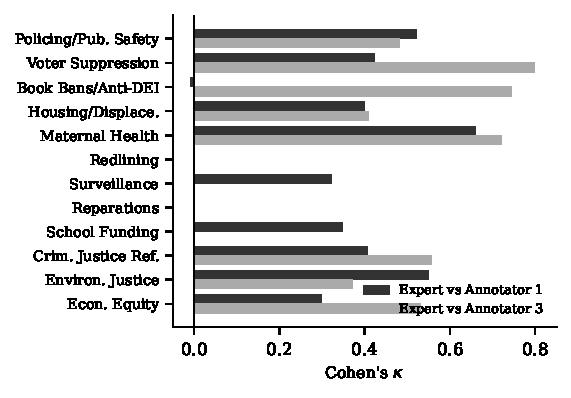
\includegraphics[width=0.9\columnwidth]{figures/fig_iaa.pdf}
\caption{Per-topic inter-annotator agreement (Cohen's $\kappa$) between
the expert re-labeling and each original annotator. Zero bars are topics
with no positive labels from either party; agreement there is undefined
in practice.}
\label{fig:iaa}
\end{figure}

\textbf{Why agreement is moderate, and why we report it anyway.} We
treat the manual annotation as a baseline standard, not perfect ground
truth, and the $\kappa$ values as a finding about the task rather than a
defect of the study. Three factors depress agreement, all visible in
Table~\ref{tab:taxonomy} and Figure~\ref{fig:iaa}. First, topic
sparsity: five topics have five or fewer positives per set, and three
have none at all in Set~3; with so few positives, a single disagreement
swings $\kappa$ dramatically, and $\kappa$ is undefined or uninformative
at zero prevalence \citep{artstein2008}. Second, feed composition: much
of the scraped stream is sports, entertainment, and lifestyle coverage
outside the taxonomy, so annotators spend most decisions confirming
absence, and the rare positive cases concentrate the ambiguity. Third,
boundary overlap: the hardest topics are those with genuinely contested
boundaries, Economic Equity absorbs stories that also touch housing or
schooling, and platform-side miscategorization (e.g., policing stories
filed under generic ``politics'') seeds anchoring disagreements. An
automated tagger evaluated against labels of this character cannot
meaningfully exceed them; it can only approach them. That is the
yardstick we adopt.

\section{Tagging Methods}
\label{sec:methods}

We evaluate six methods, in increasing order of supervision.

\textbf{Keyword tagger.} Curated seed phrases per topic, matched
against title, description, and body. High precision on explicit
mentions; blind to paraphrase.

\textbf{Semantic tagger.} Cosine similarity between the article
embedding and per-topic seed-text embeddings, using
\texttt{all-MiniLM-L6-v2} \citep{reimers2019}, with a global decision
threshold. Recovers paraphrase; noisier near the threshold.

\textbf{Hybrid OR / AND.} Union and intersection of the two base
taggers' positive sets. OR maximizes recall at heavy precision cost;
AND the reverse.

\textbf{Hybrid Soft Boost.} Keyword matches always fire; additionally,
the semantic score can fire a topic if it clears a per-topic threshold
grid-searched to maximize F1. We evaluate this in two forms. The
in-sample form tunes thresholds on the same annotator set used for
scoring; this is the version with a tuning leak, retained deliberately
as an upper bound and as a documented cautionary result. The
cross-validated (CV) form tunes thresholds on one annotator's 200
articles and applies them to the other's, eliminating the leak.

\textbf{Supervised classifier.} One logistic regression per topic
\citep{pedregosa2011}, with class-balanced weighting, over a feature
vector concatenating (i) the 384-dimensional sentence embedding of the
article text, (ii) the keyword tagger's binary decision, and (iii) the
raw semantic score for that topic. Training and testing follow the same
cross-annotator protocol as Soft Boost (CV): train on Annotator~1's
set, test on Annotator~3's, and vice versa. Topics with fewer than two
positive training examples fall back to the keyword decision; this
occurred for three topics in one direction (Redlining, Surveillance,
and Reparations, namely the zero-prevalence topics of
Table~\ref{tab:taxonomy}) and is flagged in all reported results.

\section{Evaluation}
\label{sec:eval}

\textbf{Protocol.} All methods are scored against both annotator sets
on per-topic precision, recall, F1, and Cohen's $\kappa$,
macro-averaged over the twelve topics and pooled across the two sets.
Methods requiring tuning or training never see the set they are scored
on: this cross-annotator validation is a deliberately harsh test, since
the annotators themselves agree only at $\kappa = 0.33$--$0.38$, so any
tuned artifact must survive both sampling variance and genuine
annotator shift.

\textbf{The threshold-tuning leak.} Table~\ref{tab:results} reports Soft
Boost both ways. In-sample tuning yields macro F1 0.336; the leak-free
CV form yields 0.267. The 0.07 gap (21\% of the apparent score) was
pure tuning optimism, and the honest hybrid is statistically
indistinguishable from the untuned semantic baseline (0.266). We
highlight this because per-topic threshold tuning on evaluation data is
common, tempting, and in low-prevalence regimes like ours, badly
misleading.

\begin{table}[t]
\centering
\small
\begin{tabular}{lcc}
\toprule
Method & Macro F1 & Macro $\kappa$ \\
\midrule
Keyword                    & 0.214 & 0.183 \\
Semantic                   & 0.266 & 0.225 \\
Hybrid OR                  & 0.229 & 0.181 \\
Hybrid AND                 & 0.259 & 0.244 \\
Hybrid Soft Boost (in-sample)\textsuperscript{\dag} & 0.336 & 0.297 \\
Hybrid Soft Boost (CV)     & 0.267 & 0.224 \\
\textbf{Supervised (CV)}   & \textbf{0.322} & \textbf{0.297} \\
\midrule
Human baseline (IAA)       & n/a & 0.327--0.384 \\
\bottomrule
\end{tabular}
\caption{Pooled macro-averaged results over both annotator sets.
\textsuperscript{\dag}In-sample Soft Boost tunes thresholds on the
evaluation data and is reported only as an upper bound; all other tuned
or trained methods use leak-free cross-annotator validation.}
\label{tab:results}
\end{table}

\textbf{Main result.} The supervised classifier attains macro F1 0.322
and $\kappa$ 0.297 under the leak-free protocol (Figure~\ref{fig:methods}),
a 21\% relative F1 improvement over the best honest alternative, and a
$\kappa$ equal to the \emph{leaked} Soft Boost upper bound. Measured
against the human agreement baseline, the classifier reaches 91\% of
the Set~1 ceiling ($0.297/0.327$) and 77\% of the Set~3 ceiling
($0.297/0.384$). Both cross-annotator directions agree closely (F1
0.326 testing on Set~3; 0.319 testing on Set~1), indicating the result
is not an artifact of one annotator's style.

\begin{figure*}[t]
\centering
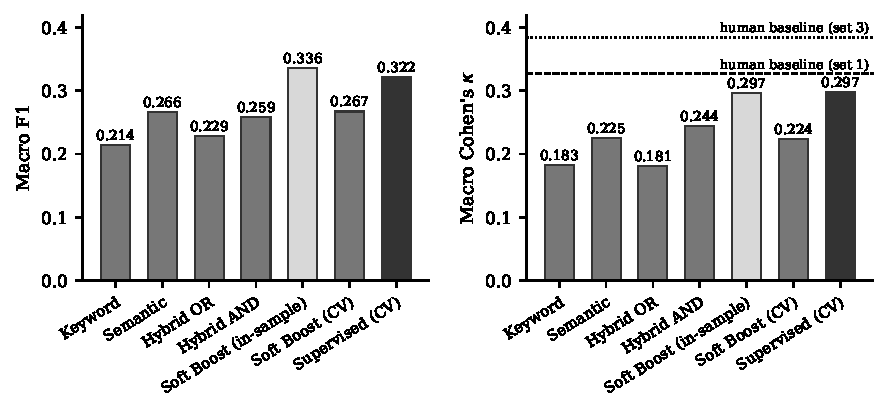
\includegraphics[width=0.8\textwidth]{figures/fig_methods.pdf}
\caption{Macro F1 (left) and Cohen's $\kappa$ (right) for all methods.
Dashed and dotted lines mark the human agreement baselines from the IAA
study. The supervised classifier (dark) is the only honest method whose
$\kappa$ approaches the human range; the in-sample Soft Boost bar (pale)
is the documented leaked upper bound.}
\label{fig:methods}
\end{figure*}

\textbf{Statistical significance.} With 200 test articles per direction
and the sparsity documented in Table~\ref{tab:taxonomy}, this gap could
plausibly be sampling noise. We test this with a paired bootstrap:
resampling the test articles with replacement (5{,}000 resamples per
direction, both methods scored on the identical resampled articles each
iteration) and recomputing the pooled macro F1 and $\kappa$ gap every
time. The F1 gap (+0.055) is positive in 98.5\% of resamples (95\% CI
$[0.005, 0.099]$, two-sided $p = 0.030$); the $\kappa$ gap (+0.073) is
positive in 99.8\% of resamples (95\% CI $[0.021, 0.118]$, two-sided
$p = 0.005$). The supervised classifier's advantage is therefore
unlikely to be a resampling artifact, though the F1 gap's interval sits
close to zero and should be read as a modest, not decisive, margin.

\textbf{Per-topic behavior.} Figure~\ref{fig:pertopic} breaks the
supervised result down by topic and direction. Performance tracks
prevalence: the well-populated topics (Economic Equity, Policing,
Housing, Criminal Justice Reform, Environmental Justice) reach F1
0.42--0.62, while the zero- and near-zero prevalence topics (Redlining,
Reparations, Surveillance) are unmeasurable: no method can be evaluated
on topics for which humans found no positive examples. We report these
as unmeasurable rather than as zeros of model quality; expanding
annotation for rare topics is future work, not a solved problem.

\begin{figure}[t]
\centering
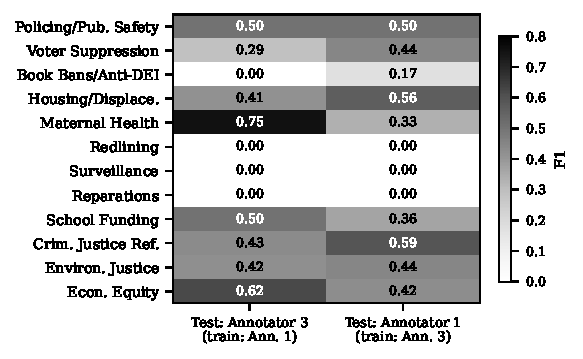
\includegraphics[width=0.9\columnwidth]{figures/fig_pertopic.pdf}
\caption{Per-topic supervised F1 in both cross-annotator directions.
Performance concentrates where human labels exist (cf.\
Table~\ref{tab:taxonomy}); blank-prevalence topics are unmeasurable.}
\label{fig:pertopic}
\end{figure}

\textbf{Production adoption.} On these results the supervised
classifier, retrained on all 400 labeled articles, replaces the keyword
matcher as the pipeline's production tagger. The frozen 400-article
benchmark and evaluation scripts run in CI, so future modifications to
the tagger or taxonomy are automatically scored against the human
baseline before deployment.

\section{Limitations and Future Work}
\label{sec:limitations}

Our efforts thus far provide evidence of the potential for increasing
the availability of diverse, representative datasets while improving
the sustainability of existing data curation practices.

\subsection{Scraping Reliability}

\textbf{JavaScript-rendered sites require brittle workarounds.} Three
of the outlets, specifically Blavity, Essence, and Capital B News, do
not expose clean server-rendered HTML or functional WordPress REST
APIs, requiring specialized scraping strategies that are inherently
more fragile than API-based approaches. Blavity, a fully
JavaScript-rendered single-page application, presented the most acute
challenges: its sitemap returns an HTML shell rather than XML,
publication dates must be recovered from embedded JSON-LD
structured-data blocks rather than raw server responses, and its CDN
occasionally serves challenge pages to automated clients that suppress
the scraper's effective yield to as few as one article per run before
the RSS fallback fires. Each of these issues independently caused the
Blavity scraper to return zero valid articles during development, and
diagnosing them required iterative live testing against the production
site. Capital B News poses a related but distinct problem: its sitemap
and category pages expose over 1,000 candidate URLs for roughly 28
articles per month, so the current implementation caps candidates at
200 and category pagination at 3 pages to keep runtime under 5 minutes,
at the cost of potentially missing older articles near the 30-day
boundary.

\textbf{Scraper fragility under site redesigns.} HTML-based scrapers
are coupled to the DOM structure of each target site. A site redesign
involving changed CSS selectors, restructured navigation, or a
migration away from WordPress will silently reduce article yield
without raising an exception. The WordPress REST API scrapers (The
Grio, The Root, NewsOne, Ebony) are comparatively robust and require no
structural DOM assumptions. We plan to add per-source yield regression
tests on a scheduled basis that alert when any source returns
significantly fewer articles than its historical baseline,
distinguishing scraper breakage from genuine low-publication periods.

\subsection{Coverage Asymmetry}

Article yield varies substantially across sources: high-cadence outlets
such as The Grio and The Root contribute approximately 300 to 400
articles per month each, while Blavity contributes approximately 30 to
35 and Capital B News approximately 50. This asymmetry means that
aggregate TF-IDF scores and topic frequency counts are dominated by the
vocabulary and coverage priorities of higher-volume outlets. Researchers
using this dataset for cross-outlet comparative analysis, or for
constructing culturally grounded AI evaluation benchmarks, should weight
or stratify by source before drawing conclusions about
community-level discourse.

\subsection{Topic Annotation Quality}

\textbf{Surface-text matching only.} The seed-phrase matcher operates
exclusively on the article title and meta-description fields.
Approximately 31\% of articles in our test window received no topic
match, reflecting both genuinely off-topic content (entertainment,
sports, culture) and cases where the relevant topic terms appear only
in the article body and not in the title or description. Full
body-text matching would substantially improve recall for the latter
group. The supervised classifier introduced in
Section~\ref{sec:methods}, which incorporates a full-text sentence
embedding rather than title/description keyword matching alone,
partially addresses this limitation for the production tagger, though
the simpler keyword and semantic taggers retain it.

\textbf{Label boundary overlap.} Seed-phrase matching produces noisy
annotations at the intersection of related topics. A story about school
segregation in a historically redlined neighborhood may legitimately
match both School Funding and Redlining \& Fair Housing; a story about
disproportionate incarceration of Black men may match both Criminal
Justice Reform and Economic Equity \& Wealth Gap. The pipeline permits
multi-label assignment, but the seed-phrase sets were defined
independently and do not encode inter-topic precedence or exclusion
rules. Future work will evaluate zero-shot classification using large
language models with the topic descriptions as natural-language
hypotheses (e.g., via a Natural Language Inference head), producing
confidence-calibrated multi-label annotations that better reflect
editorial nuance. Such an extension would also generate a valuable test
case for evaluating the cultural competence of the LLMs used as
annotators: models that lack exposure to Black press discourse may
produce systematically miscalibrated topic assignments, providing a
concrete measure of alignment quality.

\textbf{No sentiment or framing analysis.} The current pipeline
identifies \emph{what} topics are covered but not \emph{how} they are
framed. Two articles both matched to Policing \& Public Safety may take
diametrically opposed stances, one celebrating a reform, one decrying
police defunding. Extending the annotation layer with sentiment scores
or frame classifiers (e.g., using the Media Frames Corpus
\citep{card2015} as a training signal) would substantially increase the
dataset's utility both for framing studies and for constructing
culturally nuanced evaluation benchmarks for generative AI.

\subsection{Temporal and Structural Constraints}

\textbf{Rolling 30-day window.} Each pipeline run retains only articles
published within the preceding 30 days. Longitudinal analysis spanning
multiple months requires aggregating the versioned outputs across runs,
now supported by the dated-subfolder output structure, but not yet
automatically merged. A future pipeline stage will maintain a
de-duplicated cumulative corpus alongside the per-run snapshots,
enabling longitudinal studies of how Black media framing evolves and
how AI systems trained at different points diverge in cultural
alignment.

\textbf{No article body storage.} The schema stores only titles and
meta-descriptions, not full article text, to minimize storage overhead
and avoid copyright concerns around bulk reproduction of publisher
content. This limits the dataset's utility for tasks that require
body-level features, including full-text topic modeling, named entity
recognition, readability scoring, and, critically, fine-tuning of
generative AI models. We are exploring a lightweight opt-in body
extraction mode gated behind explicit researcher acknowledgment of
fair-use terms, which would substantially expand the dataset's value for
AI alignment research.

\subsection{Extensibility to Other Marginalized Ecosystems}

The pipeline's modular design, in which each source has an isolated
scraper module, a shared schema normalizer, and a declarative entry in
the publication registry, was deliberately chosen to support extension
to other under-represented publication sets whose absence from AI
training data represents distinct alignment gaps. Candidate ecosystems
include Indigenous press, Spanish-language outlets, LGBTQ+ media, and
diaspora publications, each of which contributes cultural registers,
rhetorical norms, and topic priorities that are systematically absent
from mainstream corpora. The topic taxonomy is fully configurable
through a single file (\texttt{analysis/topics.py}) with no changes
required elsewhere. However, onboarding a new outlet requires manual
investigation of its technical stack (WordPress vs.\ SPA vs.\ static
site), its URL structure, its date encoding conventions, and whether it
is accessible to automated clients, a process that took between 30
minutes (WordPress outlets) and several days (Blavity) during the
development of the current system. Reducing this onboarding friction,
for example through LLM-assisted scraper generation or scraper
templates for common CMS patterns, is a priority for future work.

\subsection{Evaluation Limitations}

\textbf{Moderate agreement, honestly reported.} Our human baseline
($\kappa$ 0.33--0.38 macro) is fair-to-moderate, and we have argued this
reflects task structure (sparsity, feed composition, boundary overlap)
rather than careless annotation. Nonetheless, all downstream numbers
inherit this uncertainty, and readers should treat per-topic scores on
sparse topics as indicative at best.

\textbf{Anchoring risk.} Original annotation sheets displayed the
keyword pipeline's predictions, which may anchor annotators toward
them; the expert re-labeling was performed blind to predictions, but the
original labels were not.

\textbf{Two annotators, one expert, and incomplete source coverage.}
The IAA study spans two annotator-expert pairs; a larger annotator pool
would tighten the baseline estimate. The annotation pool itself is also
incomplete: \emph{21ninety.com} and \emph{travelnoire.com}, two of the
ten publications the pipeline now monitors, contributed zero articles
to the 1,000-article sampling pool (Section~\ref{sec:dataset}), so
neither the annotation benchmark nor its dataset-characteristics numbers
reflect those two sources. Expanding the annotation pool to cover all
ten publications is necessary before treating this benchmark as fully
representative of the pipeline's current scope.

\textbf{No downstream experiment yet.} We validate label quality, not
downstream impact on model behavior; demonstrating that this data
measurably improves cultural alignment of a language model is the
natural next study, enabled but not performed by this work.

\section{Conclusion}

The cultural alignment of generative AI technologies depends
fundamentally on the breadth and representativeness of the data used to
build and evaluate them. Where training and evaluation corpora exclude
the media output, linguistic registers, and cultural frames of
historically marginalized communities, the resulting AI systems are
likely to underserve those communities, regardless of the sophistication
of the underlying models. Closing this gap requires, as a prerequisite,
the data infrastructure to make marginalized media content accessible
and research-ready at scale.

We have described an open-source pipeline that addresses one concrete
instance of this broader challenge: the absence of continuously updated,
community-press datasets from the Black media ecosystem, annotated
against sociologically grounded topic taxonomies, and, the central
contribution of this paper, a human-validated evaluation of that
annotation stage. A measured corpus audit grounds the motivating data
gap; a 400-article benchmark with expert re-labeling establishes a human
agreement baseline; a documented threshold-tuning leak and its
correction establish honest evaluation practice; and a supervised
classifier reaching 77--91\% of the human baseline, a margin confirmed
by a paired bootstrap significance test, becomes the production tagger
in place of the keyword matcher originally described.

We believe the architecture, comprising modular scrapers, a declarative
publication registry, an extensible topic taxonomy, and CI/CD
scheduling, together with the evaluation protocol used to validate its
tagging stage, serves as a replicable template for the data
infrastructure work that culturally aligned AI will require. The same
approach can and should be extended to other communities whose media
ecosystems are currently invisible to mainstream AI pipelines. Future
work includes broader annotation covering all ten publications, stricter
subtopic filtering as a user-facing option, and downstream experiments
measuring whether culturally grounded data of this kind improves the
alignment of generative models with the communities it represents. Code,
taxonomy, evaluation scripts, and annotation metadata (URLs, labels, and
scores; not full article text, respecting publisher copyright) will be
released upon publication.

\bibliography{aisi2027}

\end{document}
